\documentclass[0-main.tex]{subfiles}
\begin{document}

\section{Experiments}
\label{sec:expt}

\begin{table}[t!]
\vspace{5pt}
\centering
\resizebox{\linewidth}{!}{% put in textwidth
\begin{tabular}{l|l|l|l}
\hline
\rowcolor[HTML]{CBCEFB} 
                 & \multicolumn{1}{c|}{GRP}          & \multicolumn{1}{c|}{PCA} &  \multicolumn{1}{c}{CCA}           \\ \hline \hline
SIFT             &          -     & 0.443$\pm$0.008 &        -     \\ %\hline
\rowcolor[HTML]{E0E0E0} 
AlexNet conv3     & 0.559$\pm$0.018  &  0.600$\pm$0.012  &  0.494$\pm$0.006  \\ %\hline 
AlexNet conv4     & 0.568$\pm$0.007  &  0.607$\pm$0.004  &  0.488$\pm$0.005  \\ %\hline
\rowcolor[HTML]{E0E0E0} 
AlexNet pool5     & 0.565$\pm$0.008  &  0.599$\pm$0.005  &  0.486$\pm$0.012  \\ %\hline
VGG conv5\_3      & 0.571$\pm$0.005  &  \textbf{0.637$\pm$0.009}  &  0.494$\pm$0.013  \\
\rowcolor[HTML]{E0E0E0} 
VGG LCD-VLAD       & 0.506$\pm$0.001  &  0.534$\pm$0.011  &  0.523$\pm$0.010  \\ %\hline
AlexNet LCD-VLAD   & 0.517$\pm$0.001  &  0.469$\pm$0.027  &  0.534$\pm$0.018  \\
\hline
\end{tabular}
}
\caption{The silhouette score for each of the techniques and dimensionality reduction schemes on a subset of suturing demonstrations (5 expert examples). We found that PCA (100 dims) applied to VGG conv5\_3 maximizes silhouette score  \label{tab:visual}}
\vspace{-10pt}
\end{table}


\subsection{Evaluation Metrics}\label{sec:metrics}
It is important to note that \tsc is an unsupervised algorithm that does not use labeling.
Therefore, we evaluate \tsc both intrinsically (without labels) and extrinsically (against human annotations).



\vspace{0.25em}
\noindent \textbf{Intrinsic metric:} The goal of the intrinsic metric is compare the performance of different featurization techniques, encodings, and dimensionality reduction within \tsc without reference to external labels.
This score is not meant to be an absolute metric of performance but rather a relative measure.
The intrinsic metric we use measures the ``tightness" of the transition state clusters. 
This metric is meaningful since we require that each transition state cluster contains transitions from a fraction of at least $\rho$ of the demonstrations, the tightness of the clusters measures how well \tsc discovers regions of the state space where transitions are grouped together.
This is measured with the mean \textit{Silhouette Score} (denoted by \textsf{ss}), which is defined as follows for each transition state $i$:  \vspace{-5pt}
\[ \textsf{ss}(i) = \frac{b(i) - a(i)}{max\{a(i), b(i)\}},\quad \textsf{ss}(i) \in [-1,1]
\]
if transition state $i$ is in cluster $C_j$, $a(i)$ is defined the average dissimilarity of point $i$ to all points in $C_j$, and $b(i)$ the dissimilarity with the closest cluster measured as the minimum mean dissimilarity of point $i$ to cluster $C_k,\ k\neq j$. We use $L_2$-norm as the dissimilarity metric and rescale \textsf{ss} $\in[0,1]$ for ease of comparison. 

\iffalse
\begin{figure}[!t]
\centering
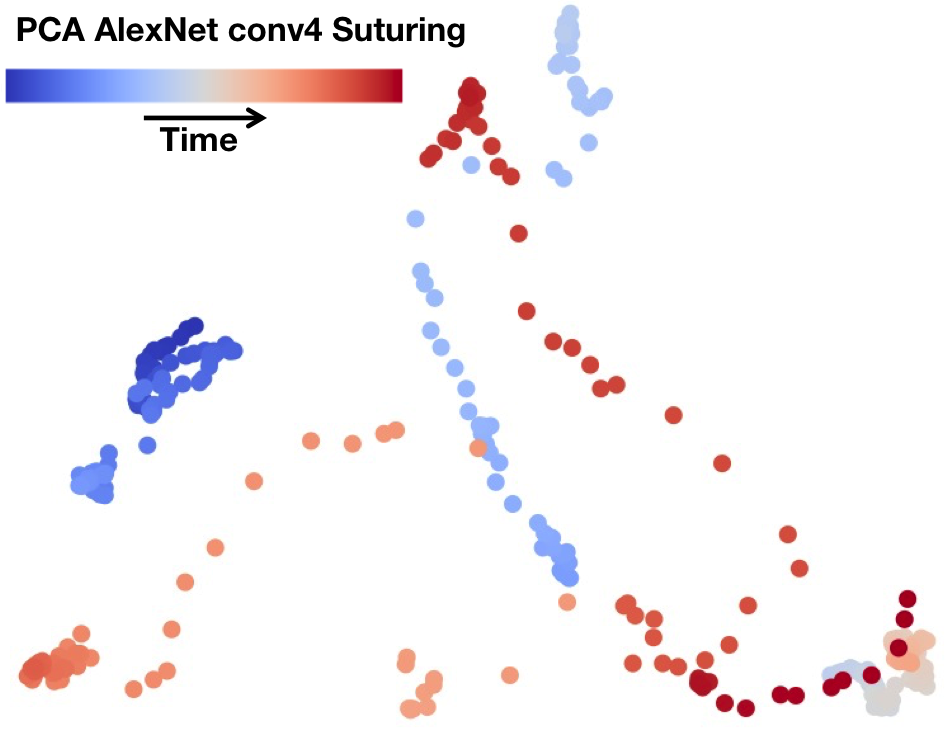
\includegraphics[width=0.5\linewidth]{figures/pca_conv4.png}
\caption{The figure visualizes the PCA projection of 64,896 dimensional output from \texttt{conv4} of the Alexnet for a sub-sequence of the suturing task video sub-sampled at 10 fps. The points are colored according to time from blue to red. We note that the visual features follow a smooth trajectory even in the high dimensional visual space. \todo{instead use a graph with knn for \% (y-axis) of time $X_{t-1}$\& $X_{t+1}$ for a given traj. at 10fps, are in k-nn with k$\in[2,30]$, rid of figure}  \label{fig:imgtraj}}
\vspace{-15pt}
\end{figure}
\fi

\begin{figure}[!b]
\vspace{-10pt}
\centering
    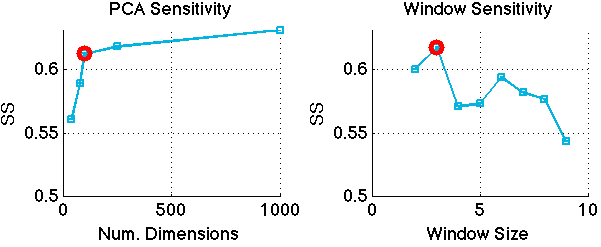
\includegraphics[width=0.95\linewidth]{figures/sensitivity}
    \caption{We evaluate the sensitivity of two hyperparameters set in advance: number of PCA dimensions and sliding window size. The selected value is shown in red double circles.\label{fig:sensitvity}}
\vspace{-10pt}
\end{figure}

\vspace{0.25em}
\noindent \textbf{Extrinsic metric:} To calculate an absolute measure of similarity of \tsc predictions $\mathcal{T}$ with respect to manual annotations $\mathcal{L}$, we use \textit{Normalized Mutual Information} (NMI) which measures the alignment between two label assignments. 
NMI is equal to the KL-divergence of the joint distribution with the product distribution of the marginals; intuitively, the distance from pairwise statistical independence.
% This metric captures the total error in alignment of predicted transitions to transitions in manual labels. 
NMI score lies in $[0,\ 1]$, where $0$ indicates independence while $1$  is perfect matching. It is defined as,
\[ NMI(\mathcal{T}, \mathcal{L}) = \frac{I(\mathcal{T}, \mathcal{L})}{\sqrt{H(\mathcal{T}) H(\mathcal{L})}}, \quad NMI(\mathcal{T}, \mathcal{L}) \in [0,1]
\]
% We compare similarity of predicted transitions to manual labels with the \textit{Dynamic Time Warping} distance between time-steps for transitions and manual labels. We normalize it by the temporal length of each example. This metric captures the total error in alignment of predicted transitions to transitions in manual labels. 

\subsection{Evaluation of Visual Featurization}
In our first experiment, we explore different visual featurization, encoding, and dimensionality reduction techniques.
We applied \tsc to our suturing experimental dataset, and measured the silhouette score of the resulting transition state clusters.
Table \ref{tab:visual} describes the featurization techniques on the vertical axis and dimensionality reduction techniques on the horizontal axis.
Our results suggest that on this dataset features extracted from the pre-trained CNNs resulted in tighter transition state clusters compared to SIFT features with a 3\% lower \textsf{ss} than the worst CNN result.
Next, we found that features extracted with the VGG architecture resulted in the highest \textsf{ss} with a 3\% higher \textsf{ss} than the best AlexNet result.
We also found that PCA for dimensionality reduction gave the best \textsf{ss} performance 7\% higher than the best GRP result and 10\% higher than best CCA result.
Because CCA finds projections of high correlation between the kinematics and video, we believe that CCA discard features informative features resulting in reduced clustering performance. 
We note that neither of the encoding schemes, VLAD or LCD\del{LCD$_{VLAD}$} significantly improve the \textsf{ss}.

\begin{figure}[!t]
\centering
%\begin{subfigure}[t]{4.4in}
    % \vspace{0pt}
    % \centering
    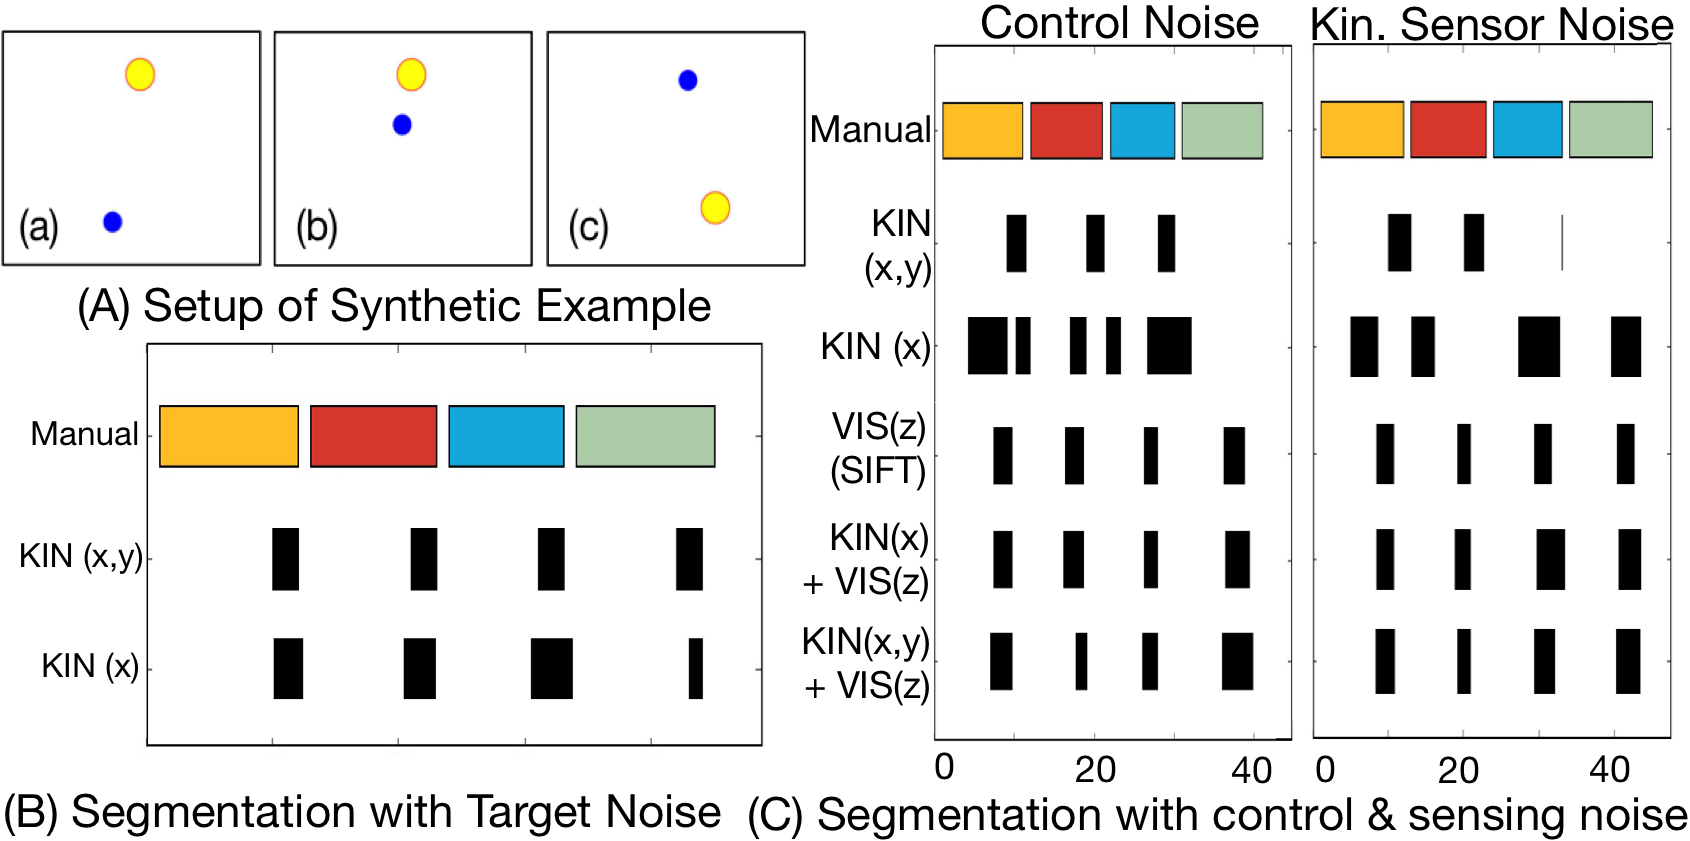
\includegraphics[width=\linewidth]{figures/toyEx-v3.png}
% 	\caption{Suturing}
% 	\par\vspace{0pt}
% 	\vspace{-15pt}
%\end{subfigure}
\caption{(A) The figure shows a 2D synthetic example with a moving point in blue and target in yellow. The robot moves to the target in a straight line in discrete steps, and a new target appears. 
(B) Segmentation results for repeated demonstrations with variance in target position.
(C) Segmentation under control noise, sensor noise, and partial observeration.}
\label{fig:toyEx}
\vspace{-10pt}
\end{figure}


There are two hyper-parameters for \tsc which we set empirically: sliding window size (T = 3), and the number of PCA dimensions (k = 100).
In Figure \ref{fig:sensitvity}, we show a sensitivity plot with the \textsf{ss} as a function of the parameter.
We calculated the \textsf{ss} using the same subset of the suturing dataset as above and with the VGG conv5\_3 CNN.
We found that T = 3 gave the best performance.
We also found that PCA with k = 1000 dimensions was only marginally better than k = 100 yet required $>$30 mins to run.
For computational reasons, we selected k = 100.




\iffalse
\subsubsection{Local Linearity of Visual Features}
In our first experiment, we explore whether the transitions state clustering model, originally derived for locally linear dynamical, is still justified for the augmented state $\mathbf{x}_(t) =\binom{k(t)}{z(t)}$.
In Figure \ref{fig:imgtraj}, for a single trajectory from one of our experimental datasets, we plot the percent if time, the points ($\mathbf{x}_(t-), \mathbf{x}_(t+1)$) lie within $k$-neighborhood of $\mathbf{x}_(t)$. We use the features from convolutional layer (\texttt{conv4}) of the pre-trained AlexNet. Higher values on y-axis for small $k$ represent that temporally consecutive points lie in vicinity in state space, even in the high dimensional visual space, supporting the assumptions of local linearity made by our model for identifying transitions.
\fi

% In Figure \ref{fig:imgtraj}, for a single trajectory from one of our experimental datasets, we plot a 2D PCA visualization of the features from convolutional layer (\texttt{conv4}) of the pre-trained AlexNet architecture. We use a sub-sequence of the full task and sub-sample the data at 10 fps and for each frame, we add a point to the visualization, illustrating the trajectory in feature space. It is worth noting that the visual features follow a smooth trajectory even in the high dimensional visual space, supporting the assumptions of local linearity made by our model for identifying transitions.

%\subsubsection{Encoding, Dimensionality Reduction, and Architecture}

\end{document}